\iffalse

Nico Casale
Cody Orazymbetov

ECE 592 HW 4

\fi

\documentclass[]{../../ncmathy}

\begin{document}

\subsection{Introduction}
	In this experiment, we implemented approximate message passing (AMP) for an $N$-length Rademacher signal, $x$. A Rademacher signal takes the following values with pmf:
	
	\begin{equation}
		f(x) = \begin{cases} 
	      \theta & if \ x = -1 \\
	      1 - 2\theta & if \ x = 0\\
	      \theta & if \ x = 1
	   \end{cases}
	\end{equation}
	
	Essentially, $2\theta$ determines the expected number of non-zeros in the signal. For instance, if $N = 2000, \theta = 0.05$, we can expect there to be roughly 200 non-zero entries in $x$. Pictured below is a stem plot that illustrates a sample of the Rademacher signal.
	
	\begin{figure}[H]
	\centering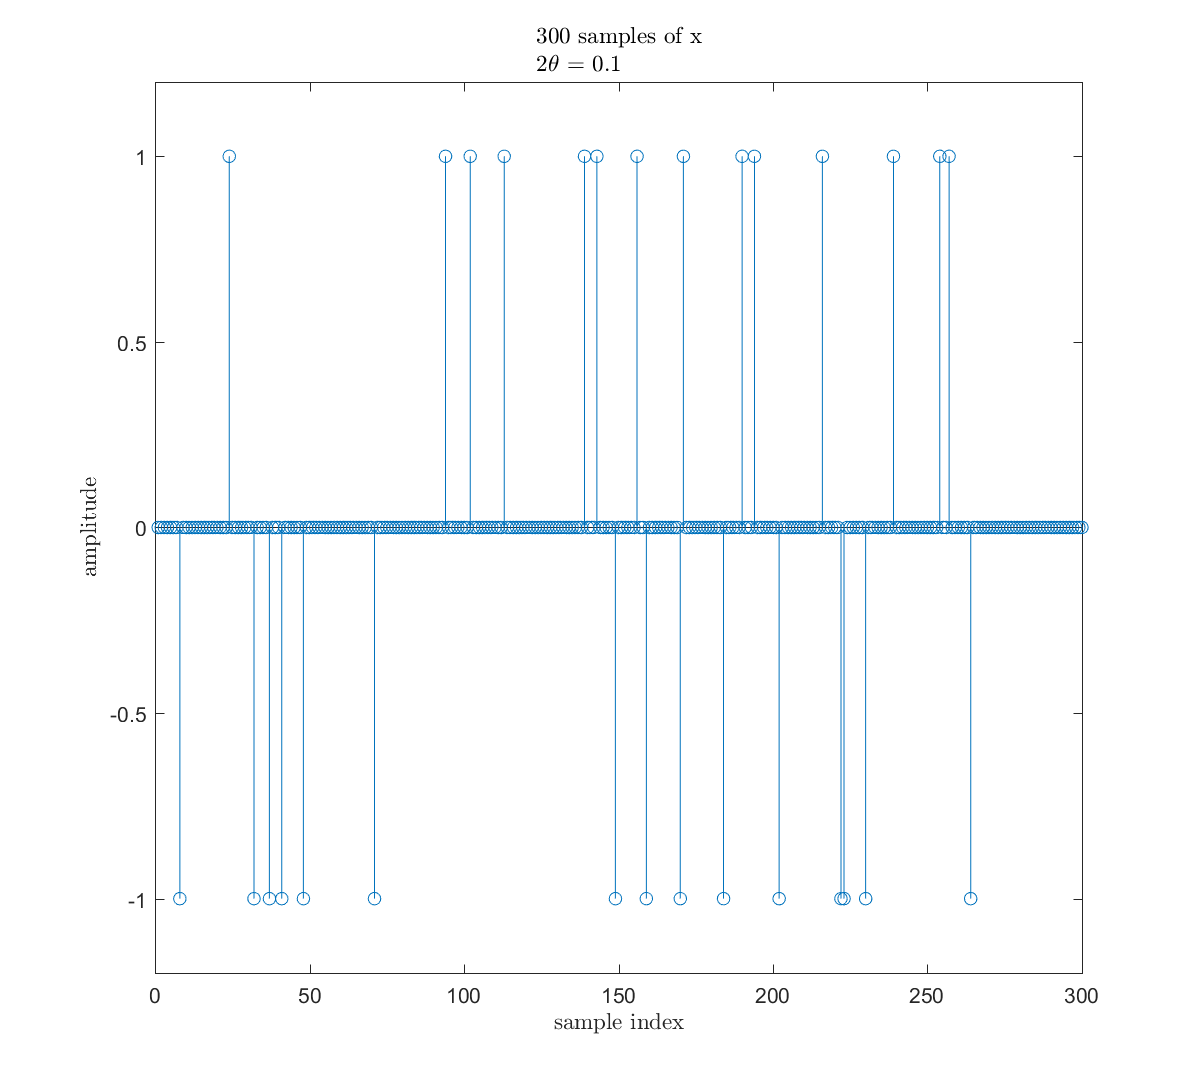
\includegraphics[width=0.6\textwidth]{rademacher}
	\caption{300 samples of the Rademacher signal.}
	\end{figure}
	
	To run AMP, we generate a measurement matrix, $A \in \mathbb{R}^{m\times n}$, where $M = round(\delta*N)$. $\delta$ is the measurement rate. In general, higher measurement rates yield a better reconstruction. We show the results of an experiment where we varied $\delta$ in section \ref{variedDelta}. Note that the elements of A are $N(0, \sqrt{\frac{1}{M}})$, which yields unit-norm columns on average.
	\\\\
	In addition, we need to generate a noise signal that disrupts the ability of AMP to reconstruct the signal. Given a signal-to-noise ratio (SNR) of $\gamma$ in dB, we generate noise $z \sim N(0,\sqrt{\gamma}) \in \mathbb{R}^{M}$. After generating the noise and measurement matrices, we can form the noisy observations, $y = Ax + z \in \mathbb{R}^{M}$. 
	
\subsection{AMP Implementation and Results}
	To complete the AMP implementation, we started with code written by Dr. Baron from the course web-page. The main modification to the script was in \code{denoise.m}, where we utilized a conditional denoiser instead of the original Weiner filter based denoiser (which is specific to denoising a Bernoulli Gaussian random variable.) The conditional expectation denoiser evaluates $E[x|v]$ as
	
	\begin{align*}
		E[x|v] &= (-1)*Pr(x=-1|v) + (0)*Pr(x=0|v) + (1)*Pr(x=1|v) \\
		&= Pr(x=1|v)-Pr(x=-1|v)
	\numberthis
	\end{align*}
	
	Where $Pr(x=1|v)$ is given by Bayes' Rule as
	
	\begin{align*}
		Pr(x=1|v) &= \frac{Pr(x=1|v)\cdot f(v)}{f(v)} \\
		&= \frac{f(x=1, v)}{f(v)} \\
		&= \frac{Pr(x=1)\cdot f(V=v|x=1)}{f(x=-1,v) + f(x=0,v) + f(x=1,v)}\\
		&= \frac{\theta\cdot\frac{1}{\sqrt{2\pi\sigma^2}}e^{\frac{-(v-1)^2}{2\sigma^2}}}{\frac{1}{\sqrt{2\pi\sigma^2}}e^{\frac{-(v+1)^2}{2\sigma^2}} + \frac{1}{\sqrt{2\pi\sigma^2}}e^{\frac{-v^2}{2\sigma^2}} + \frac{1}{\sqrt{2\pi\sigma^2}}e^{\frac{-(v-1)^2}{2\sigma^2}}}
	\numberthis
	\end{align*}
	
	Note that $Pr(x=-1|v)$ is defined similarly, albeit with $Pr(x=-1)\cdot f(V=v|x=-1) = \theta\cdot\frac{1}{\sqrt{2\pi\sigma^2}}e^{\frac{-(v+1)^2}{2\sigma^2}}$ in the numerator. Taking these quantities, $E[x|v]$ is given by
	
	\begin{align*}
		E[x|v] &= Pr(x=1|v)-Pr(x=-1|v) \\
		&= \frac{f(x=1, v) - f(x=-1, v)}{f(v)} \\
		&= \frac{Pr(x=1)\cdot f(V=v|x=1) - Pr(x=-1)\cdot f(V=v|x=-1)}{f(x=-1,v) + f(x=0,v) + f(x=1,v)}\\
		&= \frac{\theta\cdot\frac{1}{\sqrt{2\pi\sigma^2}}e^{\frac{-(v-1)^2}{2\sigma^2}} - \theta\cdot\frac{1}{\sqrt{2\pi\sigma^2}}e^{\frac{-(v+1)^2}{2\sigma^2}}}{\frac{1}{\sqrt{2\pi\sigma^2}}e^{\frac{-(v+1)^2}{2\sigma^2}} + \frac{1}{\sqrt{2\pi\sigma^2}}e^{\frac{-v^2}{2\sigma^2}} + \frac{1}{\sqrt{2\pi\sigma^2}}e^{\frac{-(v-1)^2}{2\sigma^2}}}
	\numberthis
	\end{align*}
	
	Where $\sigma$ is the variance of the Gaussian noise in $z$, $\frac{1}{\sqrt{\gamma}}$.
	\\\\
	Note that the denoiser also needs to estimate the derivative of $E[x|v]$. We do so by adding a perturbation value of $1e-10$ to each element of $v$. Then we compute $E[x|v]$ using the perturbed $v$ and calculate the piece-wise derivative as $\frac{\hat{x} - \hat{x}_{perturbed}}{perturbation}$.
	
	\subsubsection{AMP Results}
		After initializing the meta-parameters described earlier, we generate all the values and run AMP. Below is an example of our reconstruction on some samples of the input signal.
		
		\begin{figure}[H]
		\centering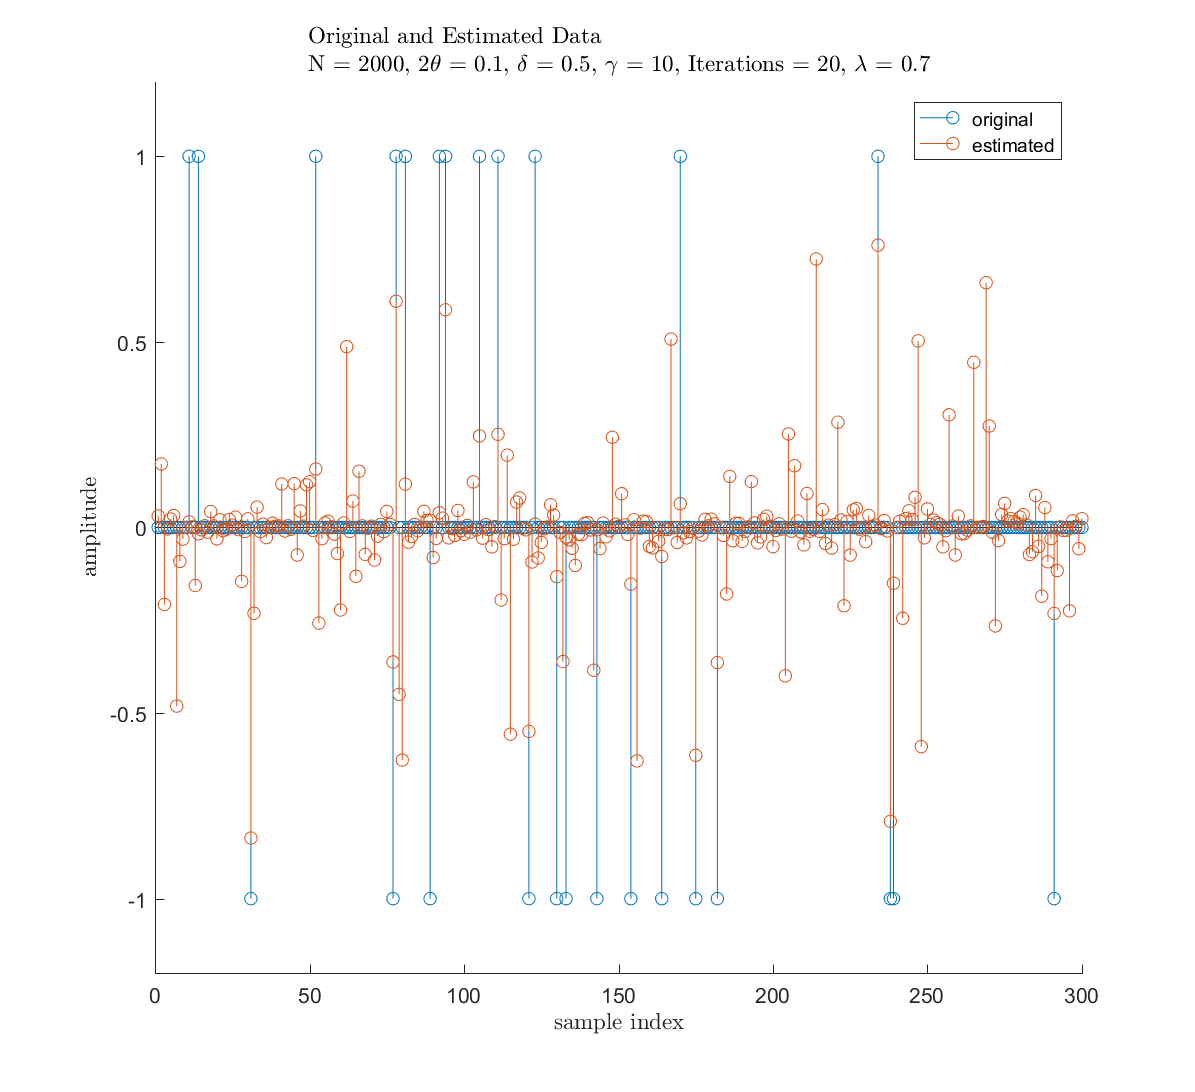
\includegraphics[width=0.6\textwidth]{AMP}
		\caption{Result of running AMP on a input signal of length $N=2000$.}
		\end{figure}

		In addition, the mean-squared error (MSE) at each iteration of the AMP algorithm is pictured below. We ran all of our simulations with 20 iterations of AMP. Note that $\lambda$ is a damping parameter that slows the update step of the estimate of $x$, $\hat{x}$. As a reminder, $2\theta$ is the probability of non-zeros in $x$, $\delta$ is the measurement rate, which is proportional to the size of $M$, and $\gamma$ is the SNR in dB, which dictates the variance (and thereby magnitude) of $z$. 
		
		\begin{figure}[H]
		\centering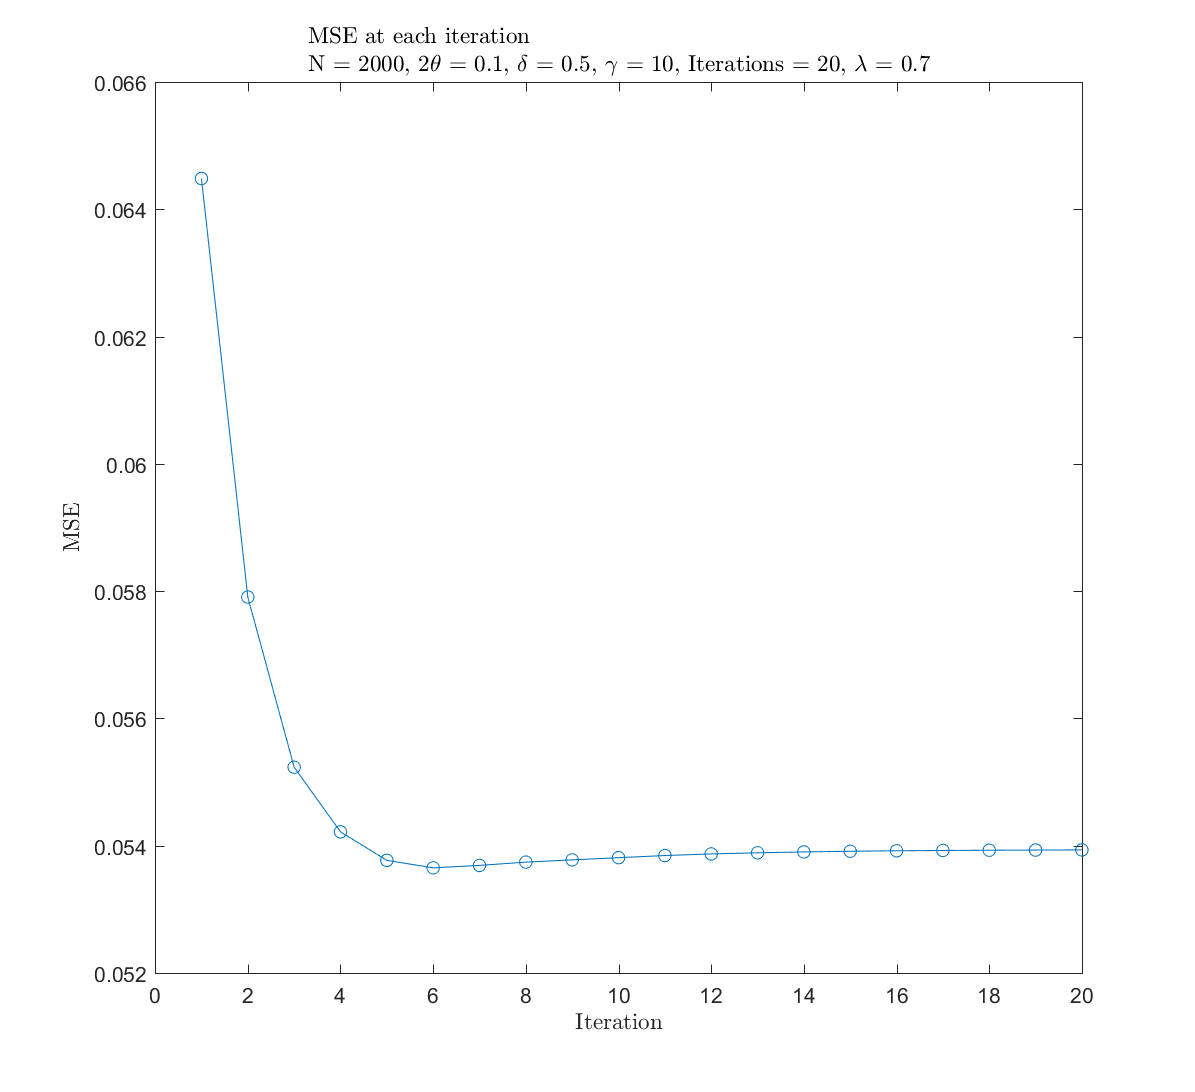
\includegraphics[width=0.6\textwidth]{AMP_mse}
		\caption{MSE at each iteration of an execution of AMP.}
		\label{incmse}
		\end{figure}	
	
\subsection{Experiments in Varying Parameters $\gamma$, $\delta$, and $N$}
	\subsubsection{Effects of Varying $\gamma$}
			For this experiment, we varied the value of $\gamma$, which is the SNR of $Ax$ with respect to the noise $z$. We find that higher SNRs yield a better reconstruction, as evidenced in the figure below. We obtained this plot by holding all parameters fixed except $\gamma$. Note that the title says `Minimum' MSE as we took only the minimum value of the MSE across the 20 iterations. On occasion, the MSE actually increases with iterations after the initial drop. This is due to variations in the noise and measurement matrices.This phenomena can be observed in fig. (\ref{incmse}).
		
		\begin{figure}[H]
		\centering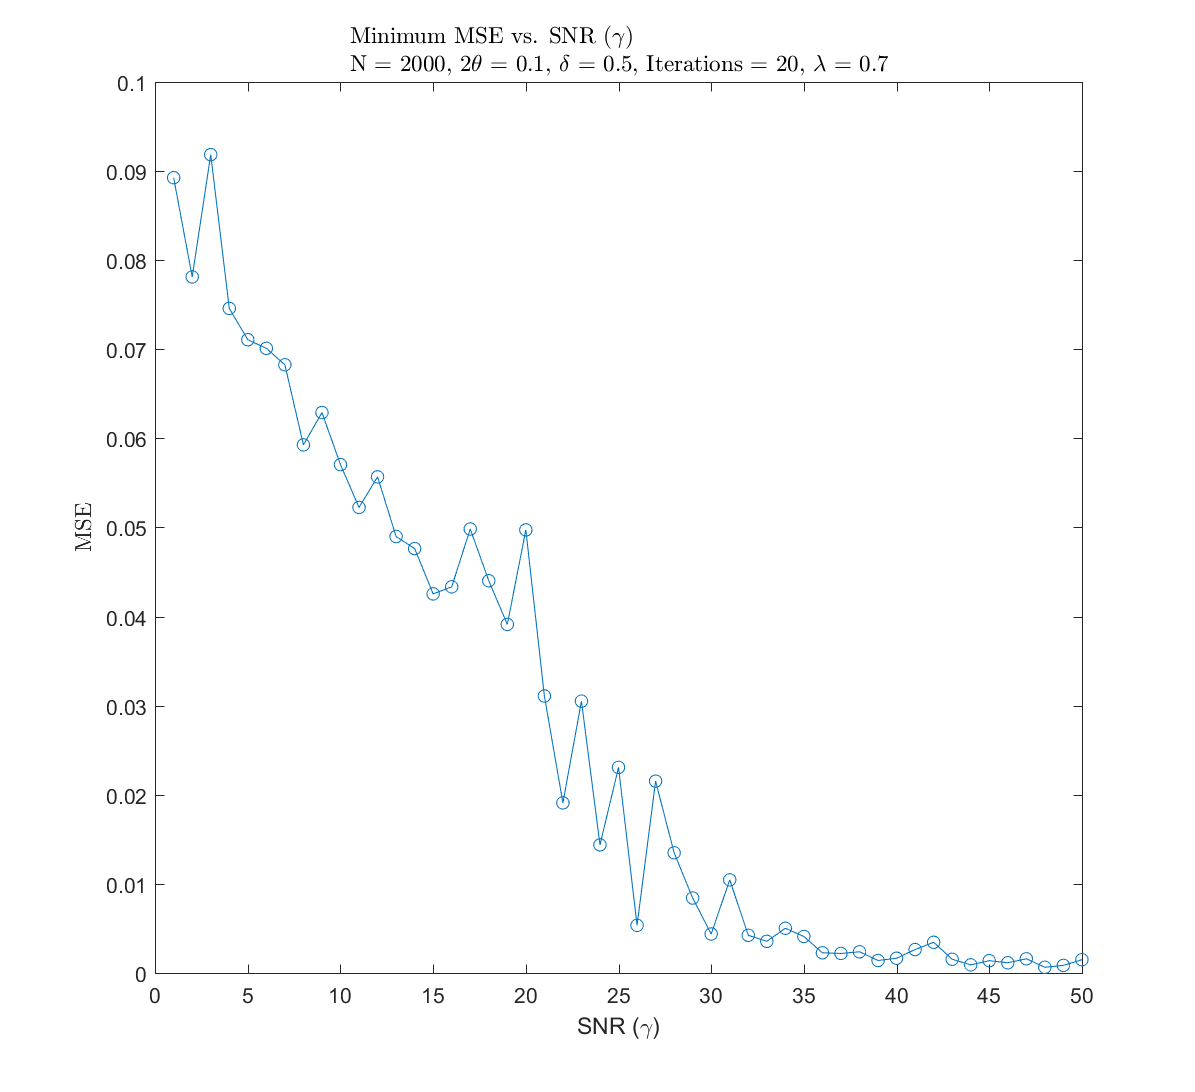
\includegraphics[width=0.6\textwidth]{vary_gamma}
		\caption{Effects of varying $\gamma$ on the MSE of AMP.}
		\end{figure}
	
	\pagebreak
	\subsubsection{Effects of Varying $\delta$} \label{variedDelta}
			For this experiment, we varied the value of $\delta$, which is the measurement rate of $A$. It determines the size in the first dimension of $A$, $M$. We find that higher measurement rates yield a better reconstruction, as evidenced in the figure below. We obtained this plot by holding all parameters fixed except $\delta$.
		
		\begin{figure}[H]
		\centering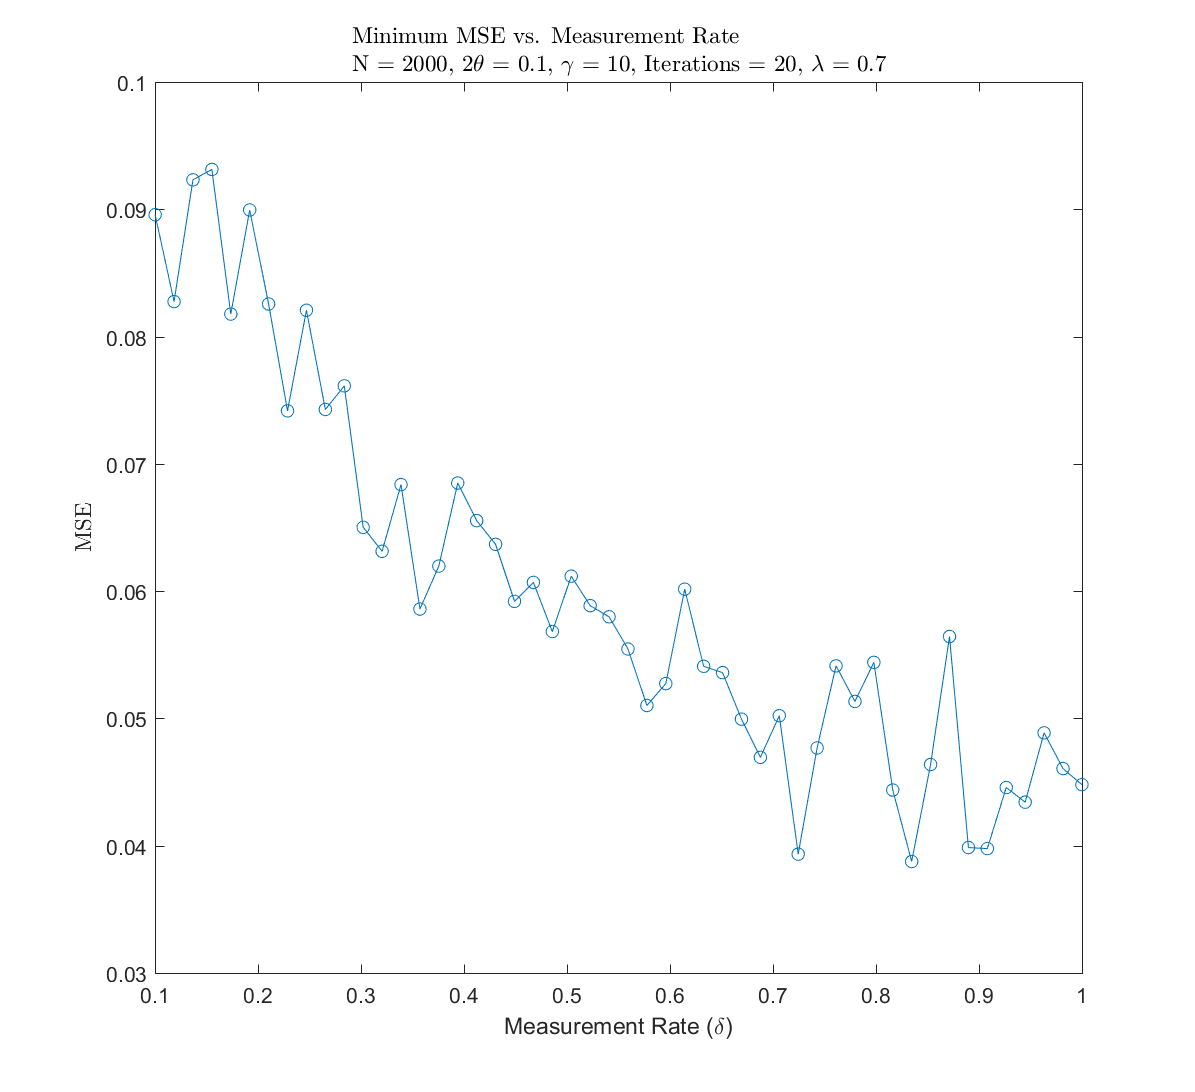
\includegraphics[width=0.6\textwidth]{vary_delta}
		\caption{Effects of varying $\delta$ on the MSE of AMP.}
		\end{figure}		
	
	\subsubsection{Effects of Varying $N$}
			For this experiment, we varied the value of $N$, which is the number of elements in $x$. It determines the size in the second dimension of $A$, $N$. We find that higher numbers of original measurements yield a better reconstruction, as evidenced in the figure below. We obtained this plot by holding all parameters fixed except $N$. Note that these values were obtained by running AMP on each value of $N$ 5 times. The average of these 5 experiments was used in the plot. This was an attempt to smooth out the plot, but as you can see it wasn't very successful. In this way, notice that the variance of the MSE between values of $N$ tends to decrease as $N$ increases. We infer that larger values of $N$ introduce more stability in the reconstruction across initialization. These larger values of $N$ are more robust to less appropriate initial values of $A$ and $z$.
		
		\begin{figure}[H]
		\centering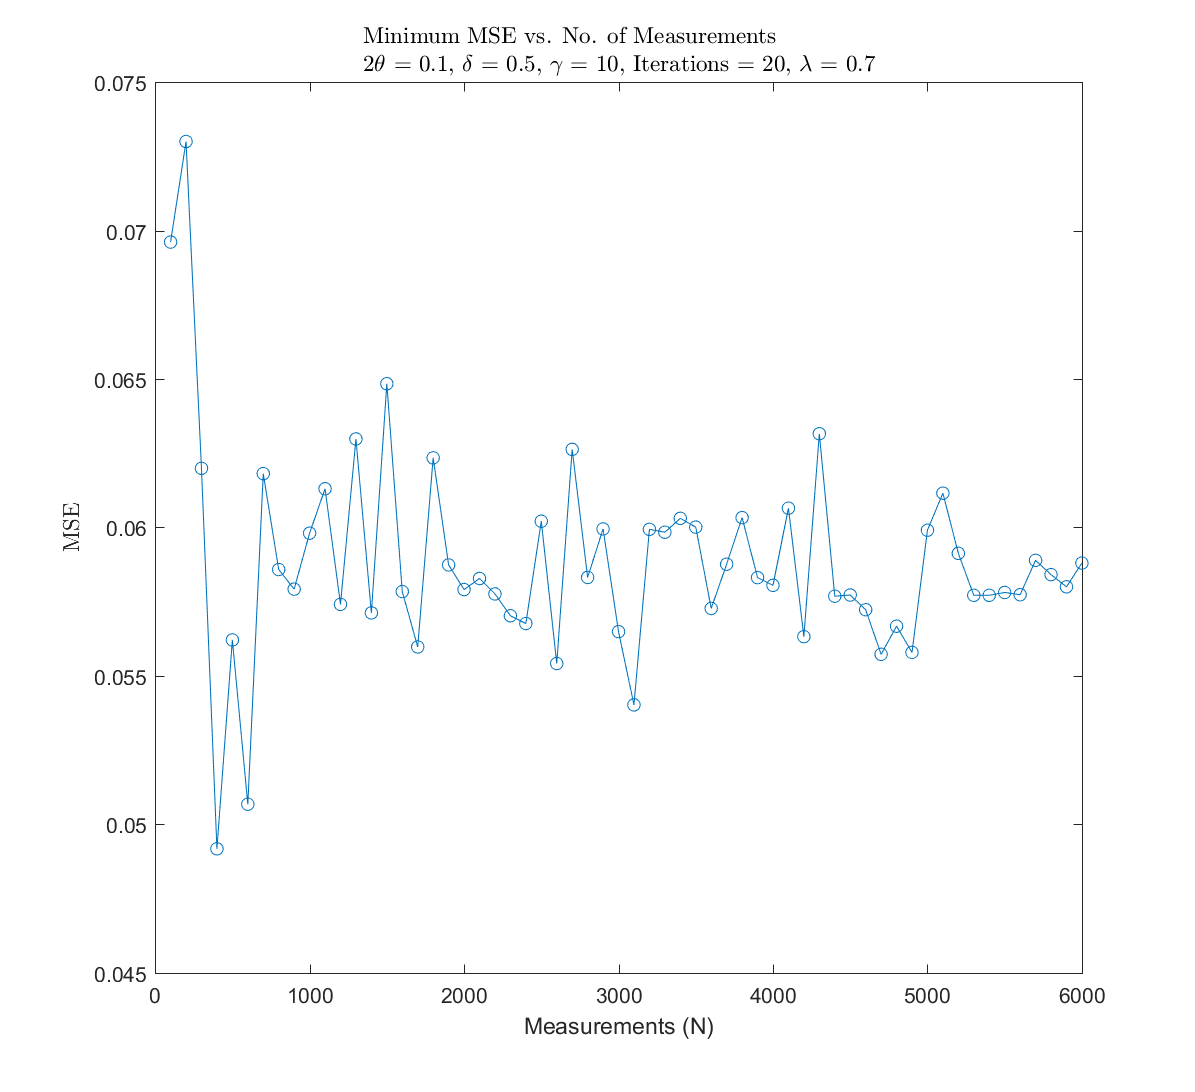
\includegraphics[width=0.6\textwidth]{vary_n}
		\caption{Effects of varying $N$ on the MSE of AMP.}
		\end{figure}		
		

\subsection{Comparison of AMP and \textit{ell-1} Recovery (Linear Programming)}
	As a final experiment, we compared the accuracy and time to execute of our AMP implementation and an implementation of ell-1 recovery. The latter is a linear programming method that utilizes the built-in MATLAB function \code{linprog(.)}. Following the example of the source code on the course website, we implemented a linear programming wrapper function that sets up the parameters to \code{linprog(.)} and returns the reconstructed signal and MSE. We captured 5 executions of AMP and ell-1 recovery for values of $N \in \{100, 200, ... , 700\}$. Below is a plot of the MSE and execution time for these experiments. Note that the time plot for AMP is at the very bottom. 
	
		\begin{figure}[H]
		\centering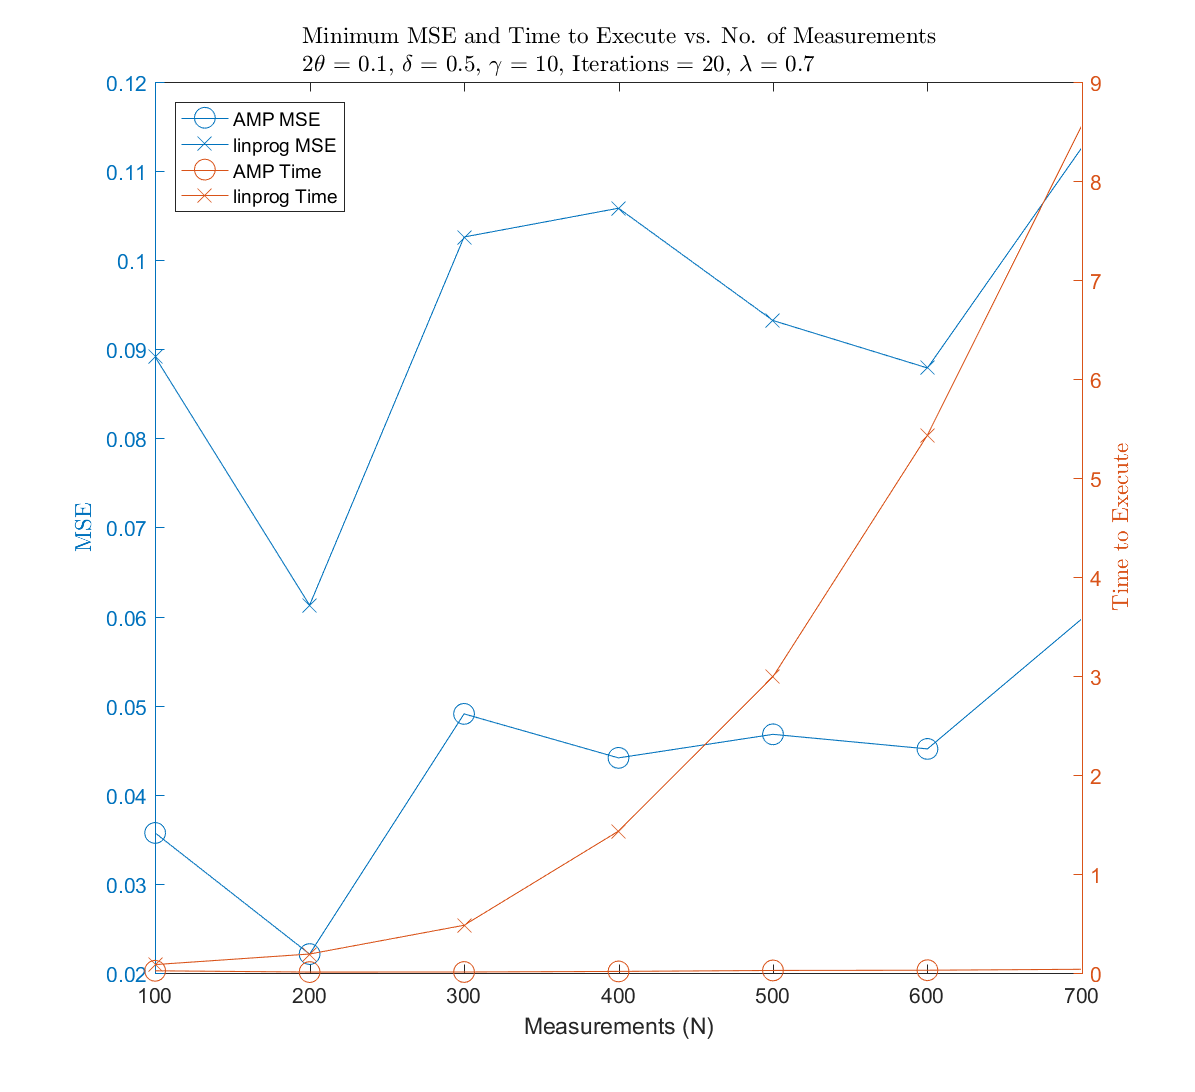
\includegraphics[width=0.6\textwidth]{ell1}
		\caption{A comparison in MSE and Time between ell-1 and AMP reconstructions.}
		\end{figure}

	We find that AMP seems to have a much better runtime compared to the linear programming implementation. The linear programming is seemingly quadratic in runtime, while the AMP seems more linear. In addition, AMP yields consistently lower MSE values than linear programming.
	
\end{document}